\section{Appendix}
\label{ch:appendix}

\subsection{Neuro-symbolic Search for Recovery Plan $\mathcal{P}$}
\label{subsec:plan}
Now, we describe our approach to solve problem (ii) as mentioned in Section~\ref{sec:problem}. Given an initial scene $S \in \mathcal{S}$ and a symbolic plan $\Pi = (\pi_1, \pi_2, .., \pi_T) \in \mathcal{P}$, the \textit{intended} intermediate states are $S_1, S_2, ..,$ and $S_T$ (see Section~\ref{sec:problem}). Using $\mathcal{T}$, $\phi$ and $S$, we can determine the corresponding \textit{intended} scene-graphs, as $Z_t = \mathcal{T}(Z_{t-1}, \pi_t)$, where $Z_0 = \phi(S)$. 

Now, assume that the first \textit{disturbance} occurred while executing $\pi_t$ on $S_{t - 1}$ resulting in a state $S_t'$, such that $S_t' \neq_\mathcal{S} S_t$. We check the equality using the learnt discriminator function $=_\mathcal{Z}$. Now our aim is to generate a plan $\Pi_{E(t)}$ such that $\mathcal{E}(S_t', \Pi_{E(t)}) =_\mathcal{S} S_k$ for some $k \leq T$. We first solve the problem of planning to an intermediate state in equivalent scene-graph space using forward-search (A$^*$) with the help of $\mathcal{T}$, $=_\mathcal{Z}$ and $\mathcal{D}$. Later, we will solve the problem of detecting the optimal intermediate state $S_k$ to plan to for \textit{fast} recovery. For the A$^*$-search, the starting state is $Z_I := \phi(S_t')$, goal-state is $Z_k$, goal-check function is $=_\mathcal{Z}$ and the heuristic function is $\mathcal{D}$. The space of actions is originally the entire $\mathcal{A}$, i.e., all symbolic action triplets of the form (\texttt{top}/\texttt{left}/\texttt{right}, $o_1$, $o_2$). However, to make the search efficient, we prune the set of actions that can be taken at any intermediate scene-graph ($Z$) using node \textit{discriminator} network, $=_\mathcal{N}$. Let the number of objects in $Z$ and $Z_k$ be $n$. Then for each $i \leq n$, we mark node as \texttt{correct} if $(o_{Z})_i =_\mathcal{Z} (o_{Z_k})_i$, and \texttt{incorrect} otherwise. Now, we use the following heuristics to prune the action space:
\vspace{-0.7em}
\begin{itemize}
    \setlength\itemsep{-0.2em}
    \item For \texttt{incorrect} nodes (say id $i$), we lookup its symbolic relation with other nodes in the goal scene-graph. This can be done either by looking at the sequence of symbolic actions $(\pi_1, \pi_2, .., \pi_k)$ leading to $Z_k$ (from $Z_0$), or by explicitly evaluating the symbolic relation using neural operator (left, right, on top etc.) on the edge embeddings in the scene-graph, $Z_k$. If it is symbolically related (say relation $a$) with some other node in the scene-graph (say id $j$), we prune all actions except $(a, i, j)$. Here $a$ is \texttt{top}, \texttt{left} or \texttt{right}. Otherwise, we prune all symbolic actions and add a new action (\texttt{mov}, $i$), which simply moves the node $i$ to its actual position in $S_k$, which is extracted from $Z_k$ via neural object bounding box decoder (see Figure~\ref{fig:sgp}).
    \item For \texttt{correct} nodes, we prune all symbolic actions.
    \item For each node (say id $i$), we add a new action (\texttt{free}, $i$), which simply moves the node $i$ to a position which is collision-free in both current and goal scene-graphs/states. Instead of explicitly reasoning over a multitude of metric positions, we learn a transformer-based neural network that predicts the required collision-free position. The learnt neural model off-loads the search over metric positions from the symbolic planner making the combined neuro-symbolic search efficient.
\end{itemize}
The action space is further pruned by using preconditions learnt for different symbolic actions. The precondition model is a neural network learnt in a supervised manner from both positive and negative examples of initial states, and uses object-relations extracted from scene-graph edges as input. For a given symbolic action, the model outputs \textit{true} if the action can be performed and \textit{false} otherwise.

\subsection{Free-Space Transformer}
To generate a collision-free position while executing "free" action on current state, we extract the bounding boxes of the objects in the current and goal scene-graphs using object bounding box decoder (in scene-graph predictor) and concatenate them together to form a single 2D tensor consisting of all the bounding boxes that the we need to avoid placing the object at. This 2D tensor along with the ID of the object to be manipulated is then passed through a transformer architecture ~\cite{Vaswani2017AttentionIA} that outputs the resulting position (bounding box) where the object should be placed to avoid collision. The network is trained on a dataset consisting of a single scene with bounding boxes for all the objects provided. We use two losses to train the network: First is an MSE Loss between the predicted bounding box and the original bounding box of the manipulated object. This loss ensures that the predicted position is in vicinity of the original position of the object and the predicted position actually represents a valid object bounding box. Second is an IoU loss that is taken between the predicted bounding box and the bounding boxes of all the objects in the scene. This loss ensures that the position is collision-free.

\begin{figure}[h!]
    \begin{subfigure}{0.5\hsize}
         \centering    
         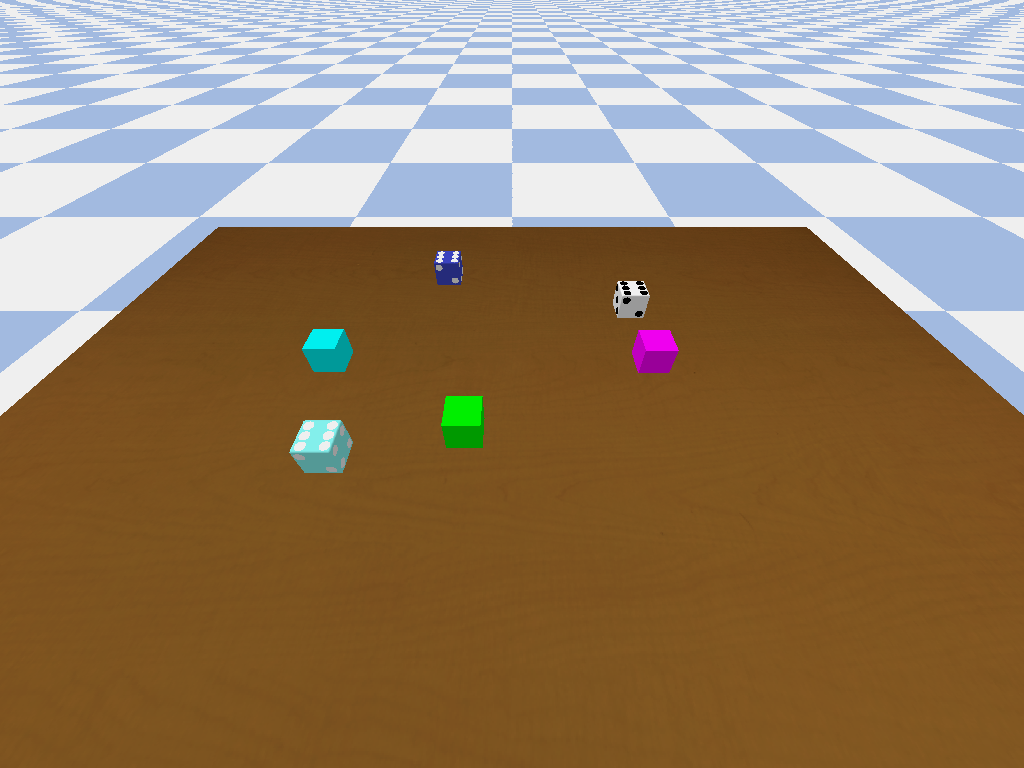
\includegraphics[scale=0.19]{figures/rze_i.png}
    \end{subfigure}
    \begin{subfigure}{0.5\hsize}
         \centering    
         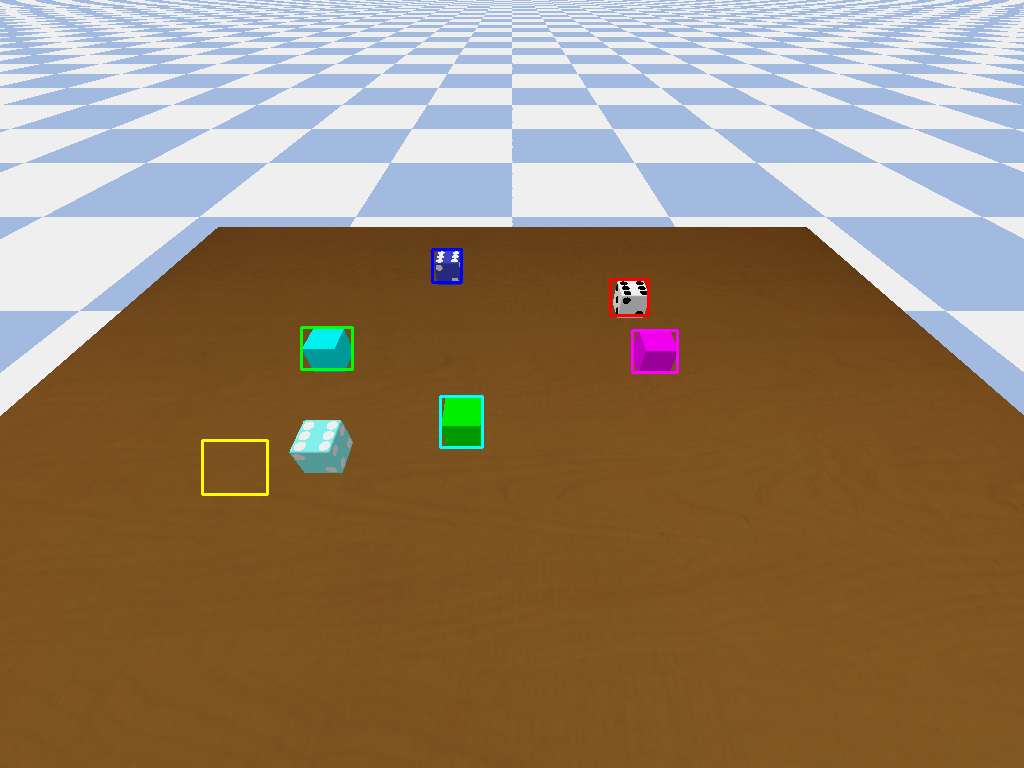
\includegraphics[scale=0.19]{figures/rze_pre.png}
    \end{subfigure}
    \caption{
        \footnotesize{
            \textbf{Output of \textit{free}-space module.} Figure on the left shows the initial scene where the task is to move the \textit{cyan lego} to a collision free position. The figure on the right shows the predicted collision free position for the \textit{cyan lego}. (yellow bounding box)
        }
    }
    \vspace{-0.15in}
    \label{fig:sgp}
\end{figure}

\subsection{Precondition Network}
To train the precondition network, we generate dataset of initial and final states and manipulation program (single action). The dataset also contains labels denoting whether the action can be executed or not (Positive/Negative examples). We extract \texttt{onTop}, \texttt{onLeft} and \texttt{onRight} relations for \textit{subject} and \textit{object} nodes for manipulation with all the other objects present in the scene. This is done by applying MLP-based networks on the edge embeddings of the scene-graph. These MLPs are trained via self-supervision on the original corpus consisting of initial and final states and single symbolic action. We pass the value of these predicates to an MLP (precondition-network) and supervise it with labels (Positive/Negative) present in the dataset. The network is trained via backpropagation of the cross-entropy loss.

\subsection{Evaluation of model components}

Table \ref{tab:model-comp} summarises the performance of various learnt networks in our model, as well the error detection and object association accuracy on the data set. Table \ref{tab:confusion} shows the confusion matrix of detection; the false positives are attributed to the sensitivity and accuracy of the scene graph discriminator.

\begin{table*}[ht]
    \begin{minipage}{.5\linewidth}
    \centering
    \caption{Accuracy of model components}
    \begin{tabular}{|l|c|}
    \hline
    Error detection & 0.96\\
    \hline
    Object association & 0.88\\
    \hline
    Scene-graph predictor & (96 \%, 0.84 IoU) \\
    \hline
    Scene-graph discriminator & 0.98\\
    \hline
    Free-space transformer & 0.007 IoU\\
    \hline
    Precondition predictor & 0.93\\
    \hline
    \end{tabular}
    \label{tab:model-comp}
    \end{minipage}
    \begin{minipage}{.5\linewidth}    
    \centering
    \caption{Confusion matrix for error detection}
    \begin{tabular}{c|r|r|}
    \multicolumn{1}{c}{}&\multicolumn{1}{c}{Predicted(P)}&\multicolumn{1}{c}{Predicted(N)}\\
    \cline{2-3}
    \multicolumn{1}{c|}{Actual(P)} & 20.5\% &  0.3\% \\
    \cline{2-3}
    \multicolumn{1}{c|}{Actual(N)} & 3.7\% & 75.5\% \\
    \cline{2-3}
    \end{tabular}
    \label{tab:confusion}
    \end{minipage}%
\end{table*}
The scores in Table~\ref{tab:model-comp} represent accuracy of the models except in case of free-space module where it represents the mean IoU of the predicted position with all other objects in the scene.



